\documentclass[11pt, a4paper, titlepage]{article}
\setlength{\parindent}{0pt}

%%%%%%%% paquetes %%%%%%%%
%\usepackage[lmargin=2cm,rmargin=2cm,top=1.5cm,bottom=2cm]{geometry}
\usepackage[T1]{fontenc}
\usepackage[utf8]{inputenc}
\usepackage[spanish,es-tabla]{babel}
\usepackage{amsmath}
\usepackage{amssymb,amsfonts,latexsym,cancel}
\usepackage{fancyhdr}
\usepackage{titlesec}
\usepackage{titling}
\usepackage{anyfontsize}
\usepackage{color}
\usepackage[dvipsnames]{xcolor}

\usepackage{csquotes}   
\usepackage[style=numeric-comp, sorting=none, block=par]{biblatex} 
\DeclareFieldFormat{title}{\bfseries\emph{#1}}
\definecolor{softblack}{RGB}{74, 71, 71} 
\DeclareFieldFormat{howpublished}{\textcolor{softblack}{\mdseries{#1}}}
\DeclareFieldFormat{labelnumberwidth}{\mkbibbold{#1\adddot}}
\setlength\bibitemsep{2.5\itemsep}
\renewcommand*{\newunitpunct}{\addspace}
\renewcommand*{\finentrypunct}{\addspace}
\usepackage{listings}
\usepackage{graphicx}
\usepackage[colorlinks = true,
			linkcolor = black,
			urlcolor = black,
			citecolor = blue ]{hyperref}

%%%%%%%% encabezado y pie de página %%%%%%%%
%\pagestyle{fancy}
%\fancyhead{}
%\fancyfoot{}
%\fancyfoot[R]{\thepage}
%\fancyfoot[L]{2º Trabajo Optimización Heurística}
%\renewcommand{\headrulewidth}{0pt}

%%%%%%%% formato de títulos y subtítulos %%%%%%%%

\definecolor{gray75}{gray}{0.75}
\newcommand{\hsp}{\hspace{20pt}}
\titleformat{\section}[hang]{\huge\bfseries}{\thesection\hsp\textcolor{gray75}{|}\hsp}{0pt}{\huge\bfseries}
\titlespacing{\section}{0pt}{0pt}{15pt}
\titleformat{\subsection}[hang]{\Large\bfseries}{\thesubsection\hsp}{0pt}{\Large\bfseries}
\titlespacing{\subsection}{0pt}{35pt}{15pt}
\titleformat{\subsubsection}[hang]{\large\bfseries}{\thesubsubsection\hspace{10pt}}{0pt}{\large\bfseries} 
\titlespacing{\subsubsection}{0pt}{20pt}{0pt}

%\titleformat{\section}[block]{\LARGE\bfseries}{\thesection.}{1mm}{}
%\titlespacing{\section}{0pc}{5.5ex}{1pc}
%\titleformat{\subsection}[block]{\Large\bfseries}{\thesubsection.}{1mm}{}
%\titlespacing{\subsection}{1.5pc}{5.5ex}{1pc}



\begin{document}

	\begin{titlepage}
    	\begin{center}
        	\hrulefill

        	\vspace{0.5cm}
        	{\bf\fontsize{25}{0}{\selectfont{Optimización Heurística\\[0.5cm]}}}
        	\fontsize{15}{0}{\selectfont{Evaluación de EAs\\[0.5cm]}}
        	\hrulefill
        	\vspace{6.0cm}
    	\end{center}

    	\centering
    	{\Large Daniel Tomás Sánchez\\ Aarón Cabero Blanco \\ Pablo Bautista 				Frías \par}
    	\vspace{2cm}
    	{\Large 08/01/2020 \par}
	\end{titlepage}

\newpage

%\renewcommand{\contentsname}{\fontsize{22}{0}{\selectfont{Índice}}}
%{\Large \tableofcontents}

\tableofcontents

\newpage

\section{Introducción}
En esta prática, el objetivo es la comparación y evaluación de diferentes algoritmos evolutivos (EAs). Para ello, además de evaluarlos, se deberá previamente  implementar un nuevo algoritmo evolutivo, el cual se explicará a continuación.
\section{Descripción del los algoritmos evolutivos}
Por un lado, se nos pidió implementar nosotros a mano un nuevo algoritmo evolutivo. Respecto al algoritmo de la práctica anterior, el actual sigue siendo un DE (Differential Evolution) pero, en este caso, se nos pidió cambiar dos operadores: el operador de cruce y el operador de mutación. En este caso, el operador de cruce es binomial, frente al exponencial de la práctica 1, y el operador de mutación es de/best/1 frente al de/rand/1 de la anterior. Este algoritmo parece ser mejor que el de la práctica anterior ya que, a la hora de realizar la mutación, se emplea el mejor genoma de la población por lo que, a primera vista, parece que convergerá más rápido.

\vspace{5mm}

Por otro lado, a la hora de elegir un algoritmo de una biblioteca que nosotros quisiéramos, nos decantamos por el SADE debido a una gran fama en su eficiencia que, como veremos después, hemos podido comprobar nosotros mismos.

\newpage

\section{Distribución del código}
El código contiene toda la parte del algoritmo implementado por nosotros y un programa principal que es el que ejecutará las funciones de esta práctica. Este programa principal, denominado $benchmarking.py$ es el encargado de realizar la funcionalidad pedida y que, tras ejecutarla, crea diferentes archivos:

\begin{itemize}
\item \textbf{benchmarking.out}: contiene los resultados de nuestro algoritmo y del SADE, en las secciones $BASIC\_DE$ y $SADE$ respectivamente, los valores estadísticos (media, mediana, min, max y desv\_est) de los dos anteriores, los resultados del test de kruskal y los fitness medios de cada función. Para consultar estos valores, como es muy extenso el archivo se recomienda abrir el archivo $benchmarking.out$.
\item \textbf{tableDE.png}: es la tabla que contiene los valores estadísticos nombrados anteriormente para cada función cuando se usa optimiza mediante nuestro DE.
\item \textbf{tableSADE.png}: es la tabla que contiene los valores estadísticos nombrados anteriormente para cada función cuando se usa optimiza mediante nuestro SADE.
\item \textbf{tableWhitney.png}: es la tabla que contiene el test de Wilcoxon comparando ambos algoritmos.
\end{itemize}
Además, se generan diferentes diagramas de caja comparando los dos algoritmos juntos por cada función.

\newpage

\section{Output de la ejecución}
En este apartado vamos a ver cuáles son las diferentes salidas que tiene nuestro código. Para ello, veremos las diferentes tablas que se generar junto con una breve descripcion explicando cada una de ellas. Además, se analizará
algún diagrama de cajas para, como dijimos antes, comparar los estadísticos típicos de los algoritmos en cada función.
\subsection{Valores estadísticos}
Aquí veremos las tablas con los valores estadísticos tanto para nuestro algoritmo como para el SADE. 

\vspace{5mm}

Hemos creado un código de color para los valores medios. Verde (los mejores) para valores menores que 1,  naranja/amarillo (los buenos/aceptables) para los valores entre 1 y 10, negro (malos/normales) para los valores entre 10 y 100 y por último rojo (muy malos) para los valores mayores que 100.
\subsubsection{Valores estadísticos DE}

\vspace{5mm}

\begin{center}
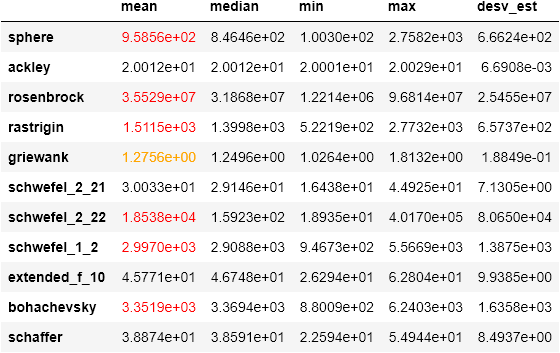
\includegraphics[width=\textwidth]{tableDE.png}
\end{center}
En esta tabla se encuentran los valores estadísticos de cada función. En casi todas ellas, los valores $min$ y $max$  se diferencian mucho del valor medio (desv\_est alta) lo que nos dice que es heterogéneo. El mejor valor medio es el de $griewank$, señalado en verde, pero esto no nos dice nada ya que son funciones diferentes que pueden converger de diferente forma. Por otro lado, la función más homogénea es la $ackley$ que se verá posteriormente.
\subsubsection{Valores estadísticos SADE}
\vspace{5mm}
\begin{center}
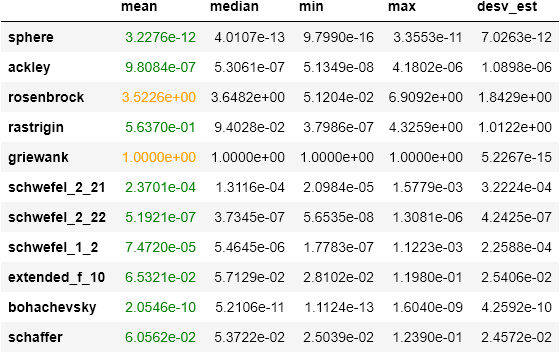
\includegraphics[width=\textwidth]{tableSADE.png}
\end{center}
Al igual que en la imagen anterior, se muestran los valores estadísticos pero, en este caso, para el SADE. Vemos que esta vez hay muchos valores medios cercanos al 0 lo que nos demuestra una mejor eficiencia del algoritmo. Por otro lado, la desv\_est es menor, cercana a 0 en casi todas las funciones que nos muestra una mayor homogeneidad de los resultados frente a los resultados obtenidos anteriormente con el DE.

\newpage

\subsection{Evaluación de EAs}
Cabe destacar que en cuanto a la evaluación de EAs, únicamente se va a realizar el test de Kruskal y el de Wilcoxon, pero no el de Friedman ya que para él es necesario un tercer algoritmo con el que comparar, cosa que no tenemos.
\subsubsection{Test de Kruskal}
\vspace{5mm}
El test de Kruskal es un test no paramétrico para probar si un grupo de datos proviene de la misma población. Se asume, bajo la hipótesis nula, que los datos vienen de la misma distribución. A continuación se muestran los datos para nuestros algoritmos:

\vspace{5mm}

Results for the sphere function: 1.3328142940540802e-09\\
Results for the ackley function: 1.3328142940540802e-09\\
Results for the rosenbrock function: 1.3328142940540802e-09\\
Results for the rastrigin function: 1.3328142940540802e-09\\
Results for the griewank function: 7.019764390051665e-10\\
Results for the schwefel\_2\_21 function: 1.3328142940540802e-09\\
Results for the schwefel\_2\_22 function: 1.3328142940540802e-09\\
Results for the schwefel\_1\_2 function: 1.3328142940540802e-09\\
Results for the extended\_f\_10 function: 1.3328142940540802e-09\\
Results for the bohachevsky function: 1.3328142940540802e-09\\
Results for the schaffer function: 1.3328142940540802e-09\\

\vspace{5mm}

Como vemos, todos ellos tienen un p-valor muy cercano al 0 lo que nos indica que los test, efectivamente, se han realizado con la misma población de datos. Además, puesto que los p-valor son muy cercanos a 0, nos denota que los fitness de las funciones tienen diferencias significativas por lo que no se puede asumir que el fitness en todas esas funciones sea el mismo. Por ello, se puede aplicar el Test de Mann Whitnet-Wilcoxon.
\newpage
\subsubsection{Test de Mann Whitney-Wilcoxon}
\vspace{5mm}
El test de Mann Whitney-Wilcoxon, al igual que el de Kruskal, es un test no paramétrico que consiste en ver si hay diferencias significativas en el comportamiento de ambos algoritmos. Para ello, se toma la hipótesis nula de que la diferencia de las medianas de las dos distribuciones es 0.

\vspace{5mm}

\begin{center}
\includegraphics[scale=0.85]{tableWhitney.png}
\end{center}

\vspace{5mm}

Como vemos en la tabla, el p-valor comparando ambos algoritmos es muy cercano a 0 y menor que el 0.05\% lo que nos ratifica que el SADE es sustancialmente mejor que nuestro DE.
\subsection{Diagramas de caja (boxplots)}
A continuación vamos a comparar los diferentes algoritmos viendo los diagramas de caja en diferentes funciones significativas. Para ello se realizarán mediante la ejecucion de 25 repeticiones, cada una de ellas con 250 iteraciones. Este pequeño número de iteraciones sirve para ver la diferencia de eficiencia y convergencia entre ambos algoritmos ya que, con estas pocas, el SADE llega al óptimo mientras que el DE no se acerca en casi ninguna de ellas.
\subsubsection{Diagrama de caja - Sphere}
\begin{center}
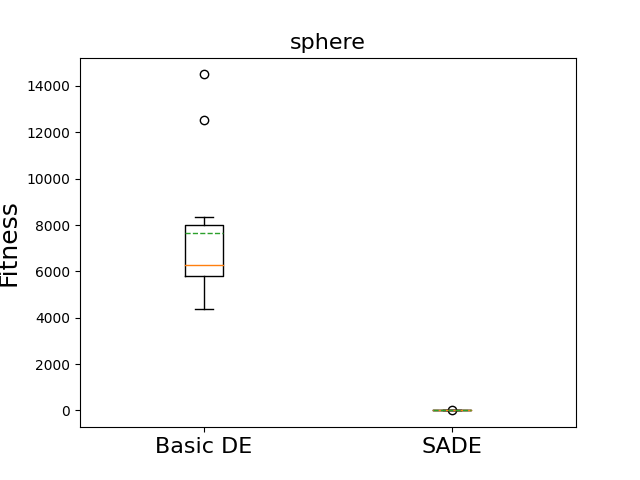
\includegraphics[scale=0.85]{sphere}
\end{center}
En la función $sphere$, se puede apreciar la diferencia de ambos algoritmos. Nuestro DE apenas se acerca al 0, con valores entre 3000 y 150, más o menos, mientras que el SADE llega perfectamente al óptimo con todos sus valores. De hecho, el diagrama de caja del SADE no se aprecia porque todos sus valores son homogéneos como vimos en las tablas mostradas anteriormente en las que la desv\_est es casi 0.
\subsubsection{Diagrama de caja - Ackley}
\begin{center}
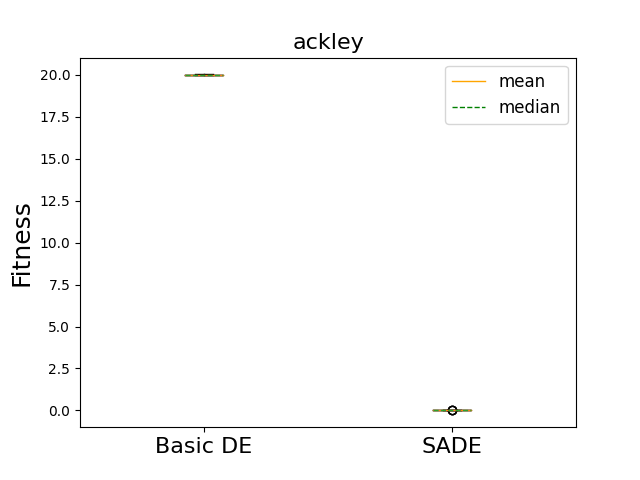
\includegraphics[scale=0.85]{ackley}
\end{center}
En esta imagen, que muestra los resultados de ambos algoritmos para la función $ackley$, podemos ver que se diferencian de 20. En este caso, el DE parece que alcanza un mínimo local ya que todos los valores están en 20, aunque se vea que, mediante el SADE, el mínimo global sea 0.
\subsubsection{Diagrama de caja - Rosenbrock}
\begin{center}
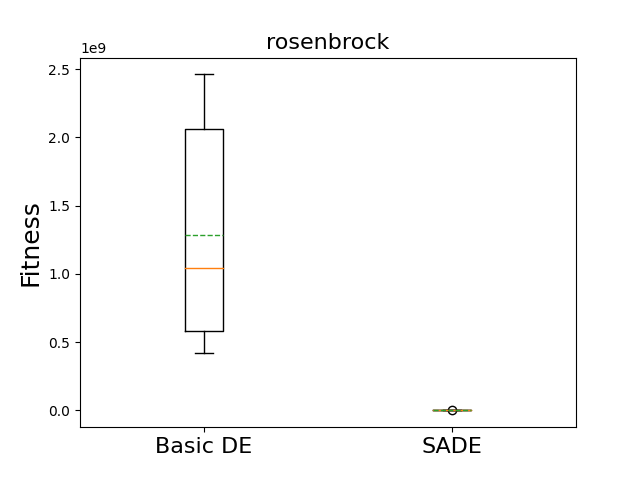
\includegraphics[scale=0.85]{rosenbrock}
\end{center}
Esta figura muestra es muy representativa ya que el DE tiene valores muy superiores al SADE, del orden de millones (véase eje y). Este comportamiento es similar al encontrado anteriormente con la función $sphere$ y a otras funciones de las que no vamos a poner diagrama porque todas se comportan prácticamente igual. Se puede seguir apreciando la diferencia de eficiencia de ambos algoritmos.
\subsubsection{Diagrama de caja - Schwefel\_2\_22}
\begin{center}
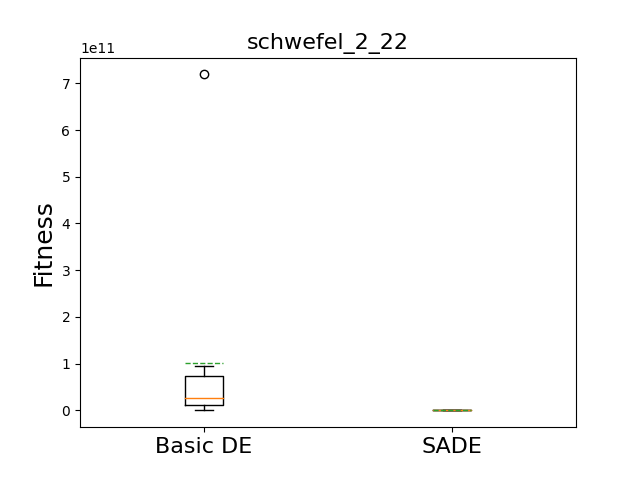
\includegraphics[scale=0.85]{schwefel_2_22}
\end{center}
Esta función es un caso aparte. Es la única que tiene valores más o menos parecidos tanto en DE como en SADE. Aunque el DE tiene gran parte de sus valores cercanos al óptimo (0), hay muchos valores atípicos muy alejados de este, lo que hace que la media se dispare y salga fuera del diagrama de caja.
\section{Conclusión}
De este trabajo hemos sacado varias conclusiones:
\begin{itemize}
\item Hay una gran diferencia de algoritmos de optimización que, por lo general, son mejores los ya implementados que los implementados por nosotros ya que son más complejos.
\item Hemos descubierto formas de comparar algoritmos que nunca antes habíamos visto.
\item Al usar diferentes librerías estadísticas, tanto para los test como para los diagramas de caja, hemos podido adentrarnos un poco en este mundillo que es muy complejo y, si a eso se le suma \LaTeX, el aprendizaje es mayor.
\end{itemize}
\end{document}
